\documentclass[12pt]{article}
\pdfoutput=1

\usepackage{amsmath}
\usepackage{amssymb,amsfonts}
\usepackage{bm}
\usepackage[mathcal]{euscript}
\usepackage[letterpaper]{geometry}
\usepackage[letterpaper]{geometry}
\usepackage{color}
\usepackage{listings}
\usepackage{natbib}
\usepackage{graphicx}
\usepackage{subfigure}
\usepackage{hyperref}

\graphicspath{{figs/}{figs_lo/}}

\definecolor{beige}{RGB}{245,245,220}

\hyphenation{ho-meo-mor-phism}
\hyphenation{ho-meo-mor-phisms}

%
% Commands
%

%\newcommand{\jlt}[1]{\textcolor{red}{(#1)}}
\newcommand{\jlt}[1]{}

\newcommand{\braidlab}{\texttt{braidlab}}%{\lstinline{braidlab}}
\newcommand{\braid}{\texttt{braid}}%{\lstinline{braid}}
\newcommand{\loopc}{\texttt{loop}}%{\lstinline{loop}}

\newcommand{\mathnotation}[2]{\newcommand{#1}{\ensuremath{#2}}}


%
% Symbols
%
\renewcommand{\l}{\left}			% \left
\renewcommand{\r}{\right}			% \right
\mathnotation{\nn}{n}				% # of strings
\mathnotation{\ac}{a}				% Dynnikov coord a
\mathnotation{\bc}{b}				% Dynnikov coord b
\mathnotation{\abv}{\bm{u}}			% Dynnikov coord vector
\mathnotation{\ip}{i}				% Counter for braid elements


\begin{document}

\lstset{language=Matlab}
\lstset{breaklines=true}
\lstset{backgroundcolor=\color{beige}}
%\lstset{emph={directory,containing,{+}braidlab},emphstyle=\color{red}}

\lstset{% general command to set parameter(s)
basicstyle=\small\ttfamily,
keywordstyle=\small\ttfamily,
identifierstyle=,
commentstyle=\small\rmfamily\itshape,%\ttfamily,
stringstyle=\small\ttfamily,
showstringspaces=false}


\title{\braidlab\ user's guide}
\author{Jean-Luc Thiffeault}
\date{}
\maketitle

\section{Installing \braidlab}

The package \braidlab\ is defined inside a Matlab namespace, which are
specified as subfolders beginning with a `\lstinline{+}' character.  The Matlab
path must contain the folder that contains the subfolder
\lstinline{+braidlab}, and not the \lstinline{+braidlab} folder
itself:
\begin{lstlisting}[frame=single,framerule=0pt,escapechar=*]
>> addpath '*\it path to folder containing +braidlab*'
\end{lstlisting}
To execute a braidlab \textit{function}, either call it using the
syntax \hbox{\lstinline{braidlab.}\textit{function}}, or import the
whole namespace:
\begin{lstlisting}[frame=single,framerule=0pt]
>> import braidlab.*
\end{lstlisting}
This allows invoking \textit{function} by itself, without the
\lstinline{braidlab} prefix.  For the remainder of this document, we
assume this has been done and omit the \lstinline{braidlab} prefix.
The \lstinline{addpath} and \lstinline{import} commands can be added
to \lstinline{startup.m} to ensure they are executed at the start of
every Matlab session.


\section{A tour of \braidlab}
\label{sec:tour}

\subsection{The \braid\ class}
\label{sec:braidclass}

\braidlab\ defines a number of classes, most importantly \braid\ and
\loopc.  The braid~$\sigma_1\sigma_2^{-1}$ is defined by
\begin{lstlisting}[frame=single,framerule=0pt]
>> a = braid([1 -2])   % defaults to 3 strings

a = < 1 -2 >
\end{lstlisting}
which defaults to the minimum required strings,~$3$.  The same braid
on~$4$ strings is defined by
\begin{lstlisting}[frame=single,framerule=0pt]
> a4 = braid([1 -2],4)   % force 4 strings

a4 = < 1 -2 >
\end{lstlisting}
Two braids can be multiplied:
\begin{lstlisting}[frame=single,framerule=0pt]
>> a = braid([1 -2]); b = braid([1 2]);
>> a*b, b*a

ans = < 1 -2  1  2 >

ans = < 1  2  1 -2 >
\end{lstlisting}
Powers can also be taken, including the inverse:
\begin{lstlisting}[frame=single,framerule=0pt]
>> a^5, inv(a), a*a^-1

ans = < 1 -2  1 -2  1 -2  1 -2  1 -2 >

ans = < 2 -1 >

ans = < 1 -2  2 -1 >
\end{lstlisting}
Note that this last expression is the identity braid, but is not
simplified.  The method \lstinline{compact} attempts to simplify the
braid:
\begin{lstlisting}[frame=single,framerule=0pt]
>> compact(a*a^-1)

ans = < e >
\end{lstlisting}
The method \lstinline{compact} is based on the heuristic algorithm
of~\cite{Bangert2002}, since finding the braid of minimum length in
the standard generators is in general difficult~\citep{Paterson1991}.

The number of strings is
\begin{lstlisting}[frame=single,framerule=0pt]
>> a.n

ans = 3
\end{lstlisting}
Note that
\begin{lstlisting}[frame=single,framerule=0pt]
>> help braid
\end{lstlisting}
describes the class \braid.  To get more information on the \braid\
constructor, invoke
\begin{lstlisting}[frame=single,framerule=0pt]
>> help braid.braid
\end{lstlisting}
which refers to the method \braid\ within the class \braid.  (Use
\lstinline{methods(braid)} to list all the methods in the class.)
There are other ways to construct a \braid, such as using random
generators, here a braid with~$5$ strings and~$10$ random generators:
\begin{lstlisting}[frame=single,framerule=0pt]
>> braid('random',5,10)

ans = < 1  4 -4  2  4 -1 -2  4  4  4 >
\end{lstlisting}
The constructor can also build some standard braids:
\begin{lstlisting}[frame=single,framerule=0pt]
>> braid('halftwist',5)

ans = < 4  3  2  1  4  3  2  4  3  4 >
\end{lstlisting}
In Section~\ref{sec:braidfromdata} we will also show how to construct
a braid from a trajectory data set.

The \braid\ class also handles equality of braids:
\begin{lstlisting}[frame=single,framerule=0pt]
>> a = braid([1 -2]); b = braid([1 -2 2 1 2 -1 -2 -1]);
>> a == b

ans = 1
\end{lstlisting}
These are the same braid.  Equality is determined efficiently by
acting on loop (Dynnikov) coordinates~\citep{Dynnikov2002}, as
described by \citet{Dehornoy2008}.  See
Sections~\ref{sec:loop}--\ref{sec:loopcoords} for more details.

We can extract a subbraid by choosing specific strings: for example,
if we take the~$4$-string braid~$\sigma_1\sigma_2\sigma_3^{-1}$ and
discard the third string, we obtain~$\sigma_1\sigma_2^{-1}$:
\begin{lstlisting}[frame=single,framerule=0pt]
>> a = braid([1 2 -3]);
>> subbraid(a,[1 2 4])   % subbraid using strings 1,2,4

ans = < 1 -2 >
\end{lstlisting}

There are a few methods that exploit the connection between braids and
homeomorphisms of the punctured disk.  Braids label \emph{isotopy
  classes} of homeomorphisms, so we can assign a topological entropy
to a braid:
\begin{lstlisting}[frame=single,framerule=0pt]
>> entropy(braid([1 2 -3]))

ans = 0.8314
\end{lstlisting}
The entropy is computed by iterated action on a
loop~\citep{Moussafir2006}.  This can fail if the braid is
finite-order or has very low entropy:
\begin{lstlisting}[frame=single,framerule=0pt]
>> entropy(braid([1 2]))
Warning: Failed to converge to requested tolerance; braid is likely finite-order or has low entropy. 
> In braid.entropy at 89

ans = 0
\end{lstlisting}
To force the entropy to be computed using
the Bestvina--Handel train track algorithm~\cite{Bestvina1995}, we add
an optional parameter:
\begin{lstlisting}[frame=single,framerule=0pt]
>> entropy(braid([1 2]),'trains')

ans = 0
\end{lstlisting}
Note that for large braids the Bestvina--Handel algorithm is
impractical.  But when applicable it can also determine the
Thurton--Nielsen type of the
braid~\citep{Fathi1979,Thurston1988,Casson1988,Boyland1994}:
\begin{lstlisting}[frame=single,framerule=0pt]
>> tntype(braid([1 2 -3]))

ans = pseudo-Anosov
>> tntype(braid([1 2]))

ans = finite-order
>> tntype(braid([1 2],4))  % reducing curve around 1,2,3

ans = reducible
\end{lstlisting}
\braidlab\ uses Toby Hall's implementation of the Bestvina--Handel
algorithm~\citep{HallTrain}.

Finally, we can also find the Burau matrix
representation~\citep{Burau1936,Birman1975} of a braid:
\begin{lstlisting}[frame=single,framerule=0pt]
>> burau(braid([1 -2]),-1)

ans = 1    -1
     -1     2
\end{lstlisting}
where the last argument ($-1$) is the value of the parameter~$t$ in
the Laurent polynomials that appear in the entries of the Burau
matrices.


\subsection{Constructing a braid from data}
\label{sec:braidfromdata}

One of the main purposes of \braidlab\ is to analyze two-dimensional
trajectory data using braids.  We can assign a braid to trajectory
data by looking for \emph{crossings} along a projection
line~\citep{Thiffeault2005,Thiffeault2010}.  The \braid\ constructor
allows us to do this easily.

The folder \lstinline{testing} contains a dataset of trajectories,
from laboratory data for granular media~\cite{Puckett2012}.  From the
\lstinline{testing} folder, we load the data:
\begin{lstlisting}[frame=single,framerule=0pt]
>> clear; load testdata
>> whos
  Name         Size               Bytes  Class     Attributes

  XY        9740x2x4             623360  double              
  ti           1x9740             77920  double              
\end{lstlisting}
Here \lstinline{ti} is the vector of times, and \lstinline{XY} is a
three-dimensional array: its first component specifies the timestep,
its second specifies the $X$ or $Y$ coordinate, and its third
specifies one of the~$4$ particles.  Figure~\ref{fig:testdata_trajs3}
shows
%
\begin{figure}
\begin{center}
\subfigure[]{
  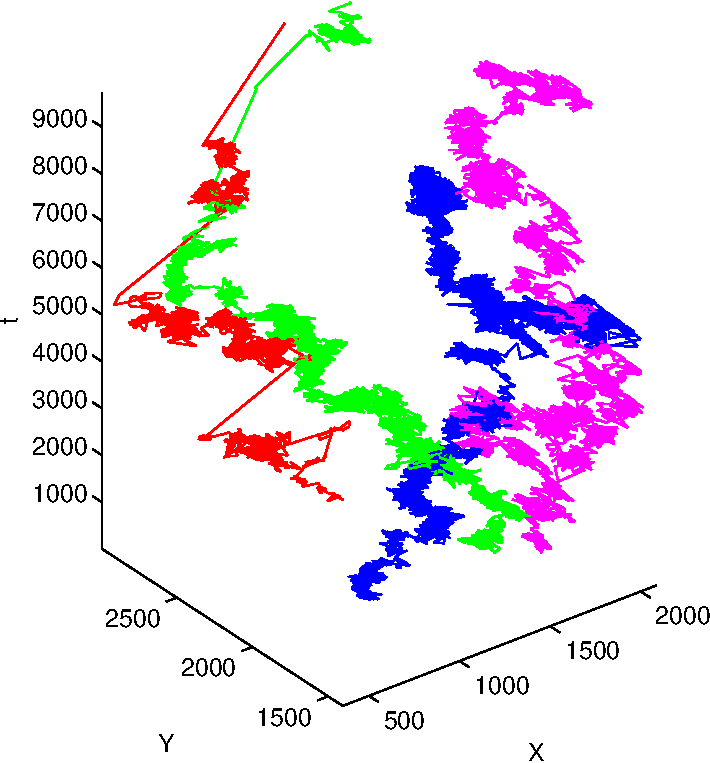
\includegraphics[height=.3\textheight]{testdata_trajs3}
  \label{fig:testdata_trajs3}
}\hspace{1em}
\subfigure[]{
  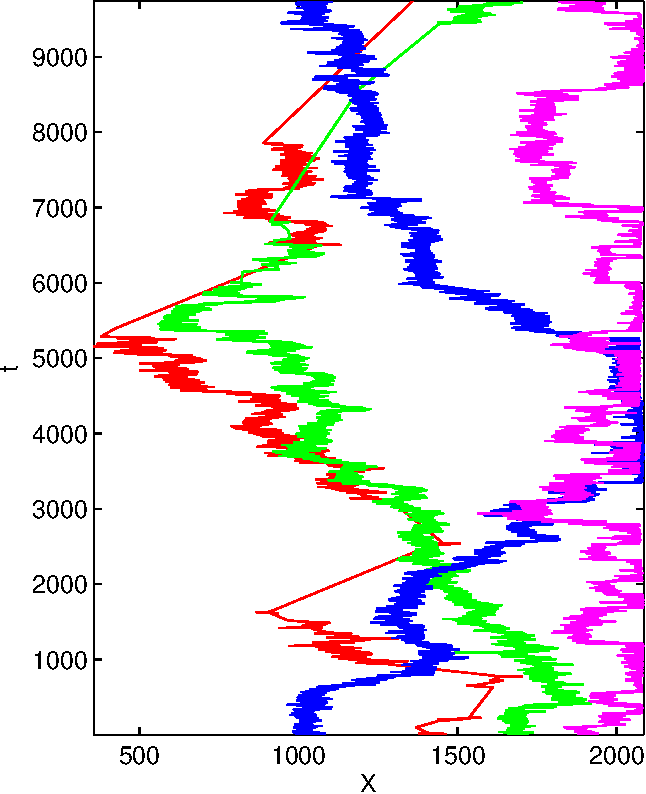
\includegraphics[height=.3\textheight]{testdata_trajs}
  \label{fig:testdata_trajs}
}\hspace{1em}
\subfigure[]{
  
\includegraphics[height=.3\textheight]{testdata_braid}
  \label{fig:testdata_braid}
}\hspace{1em}
\subfigure[]{
  
\includegraphics[height=.3\textheight]{testdata_braidY}
  \label{fig:testdata_braidY}
}
\end{center}
\caption{(a) A dataset of four trajectories, (b) projected alond
  the~$X$ axis.  (c) The compacted braid~$ \sigma_1^{-1} \sigma_2^{-1}
  \sigma_1^{-8}\sigma_3^2\sigma_2\sigma_1$ corresponding to the~$X$
  projection in (b).  (d) The compacted
  braid~$\sigma_3^{-7}\sigma_1\sigma_3^{-1}\sigma_1$ corresponding to
  the~$Y$ projection, with closure enforced.  The braids in (c) and
  (d) are conjugate.}
\end{figure}
%
the~$X$ and~$Y$ coordinates of these four trajectories, with time
plotted vertically.  Figure~\ref{fig:testdata_trajs} shows the same
data, but projected along the~$X$ direction.  To construct a braid
from this data, we simply execute
\begin{lstlisting}[frame=single,framerule=0pt]
>> b = braid(XY);
>> b.length

ans = 894
\end{lstlisting}
This is a very long braid!  But Figure~\ref{fig:testdata_trajs}
suggests that this is misleading: many of the crossings are `wiggles'
that cancel each other out.  Indeed, if we attempt to shorten the
braid:
\begin{lstlisting}[frame=single,framerule=0pt]
>> b = compact(b)

b = < -1 -2 -1 -1 -1 -1 -1 -1 -1 -1  3  3  2  1 >
>> b.length

ans = 14
\end{lstlisting}
we find the number of generators (the length) has dropped to~$14$!  We
can then plot this shortened braid as a braid diagram using
\lstinline{plot(b)} to produce Figure~\ref{fig:testdata_braid}.  The
braid diagram allows us to see topological information clearly, such
as the fact that the second and third particles undergo a large number
of twists around each other; we can check this by creating a subbraid
with only those two strings:
\begin{lstlisting}[frame=single,framerule=0pt]
>> subbraid(bX,[2 3])

ans = < -1 -1 -1 -1 -1 -1 -1 -1 >
\end{lstlisting}
which shows that the winding number between these two strings is~$-4$.

The braid was constructed from the data by assuming a projection along
the~$X$ axis (the default).  We can choose a different projection by
specifying an optional angle for the projection line; for instance, to
project along the~$Y$ axis we invoke
\begin{lstlisting}[frame=single,framerule=0pt]
>> b = braid(XY,pi/2);   % project onto Y axis
>> b.length

ans = 673
>> b.compact

ans = < -3 -3 -3 -3 -3 -3 -3  1 -3 >
\end{lstlisting}
In general, a change of projection line only changes the braid by
conjugation~\citep{Boyland1994,Thiffeault2010}.  We can test for
conjugacy:
\begin{lstlisting}[frame=single,framerule=0pt]
>> bX = compact(braid(XY,0)); bY = compact(braid(XY,pi/2));
>> conjtest(bX,bY)   % test for conjugacy of braids

ans = 0
\end{lstlisting}
The braids are not conjugate.  This is because our trajectories do not
form a `true' braid: the final points do not correspond exactly with
the initial points, as a set.  If we truly want a
rotationally-conjugate braid out of our data, we need to enforce a
closure method:
\begin{lstlisting}[frame=single,framerule=0pt]
>> XY = closure(XY);   % close braid and avoid new crossings
>> bX = compact(braid(XY,0)), bY = compact(braid(XY,pi/2))

bX = < -1 -2 -1 -1 -1 -1 -1 -1 -1 -1  3  3  2  1 >

bY = < -3 -3 -3 -3 -3 -3 -3  1 -3  1 >
\end{lstlisting}
This default closure simply draws line segments from the final points
to the initial points in such a way that no new crossings are created
in the~$X$ projection.  Hence, the $X$-projected braid \lstinline{bX}
is unchanged by the closure, but here the $Y$-projected braid
\lstinline{bY} is longer by one generator (\lstinline{bY} is plotted
in Figure~\ref{fig:testdata_braidY}).  This is enough to make the
braids conjugate:
\begin{lstlisting}[frame=single,framerule=0pt]
>> [~,c] = conjtest(bX,bY)  % ~ means discard first return arg

c = < 3  2 >
\end{lstlisting}
where the optional second argument \lstinline{c} is the conjugating
braid, as we can verify:
\begin{lstlisting}[frame=single,framerule=0pt]
>> bX == c*bY*c^-1

ans = 1
\end{lstlisting}
There are other ways to enforce closure of a braid (see
\lstinline{help closure}), in particular
\lstinline{closure(XY,'mindist')}, which minimizes the total distance
between the initial and final points.

Note that \lstinline{conjtest} uses the library \emph{CBraid}
\citep{CBraid} to first convert the braids to Garside canonical
form \citep{Birman2005}, then to determine conjugacy.  This is very
inefficient, so is impractical for large braids.


\subsection{The \loopc\ class}
\label{sec:loop}

A simple closed loop on a disk with~$5$ punctures is shown in
Figure~\ref{fig:dynn_loop}.
%
\begin{figure}
\begin{center}
\subfigure[]{
  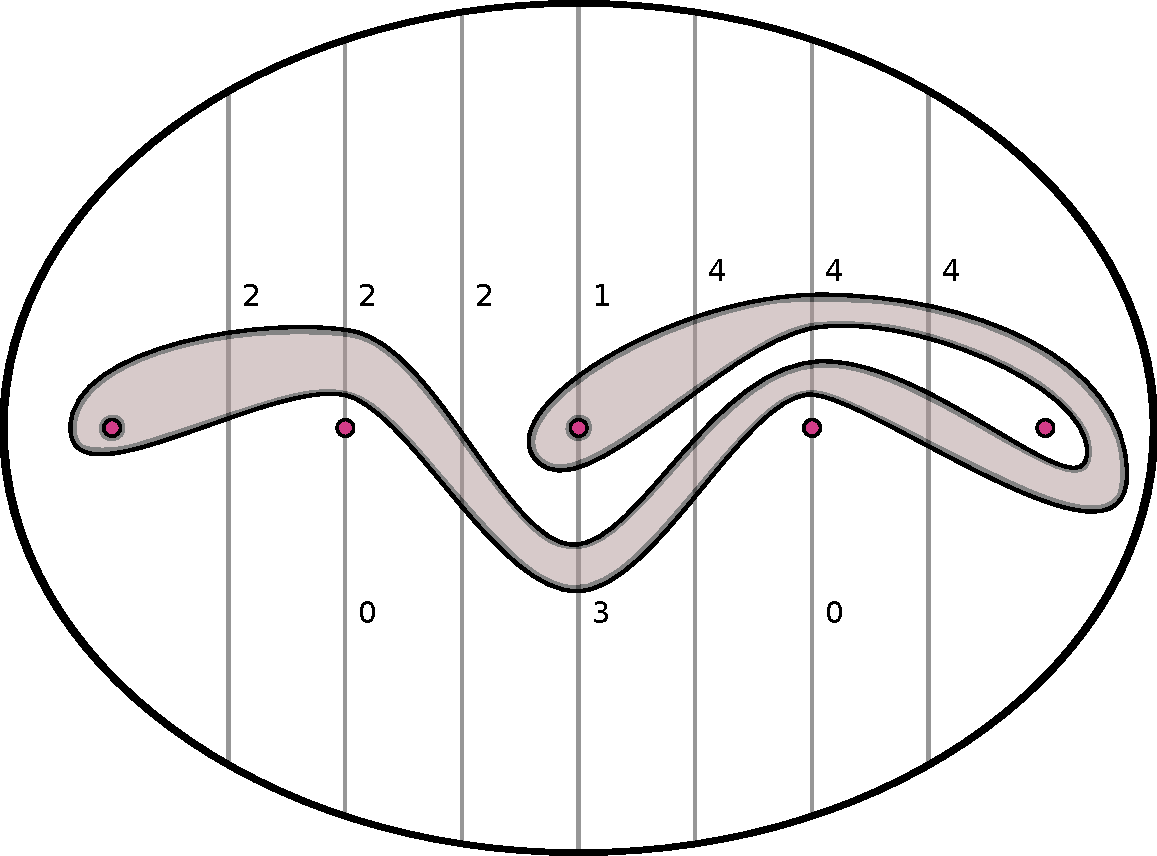
\includegraphics[height=.22\textheight]{dynn_loop}
  \label{fig:dynn_loop}
}\hspace{1em}
\subfigure[]{
  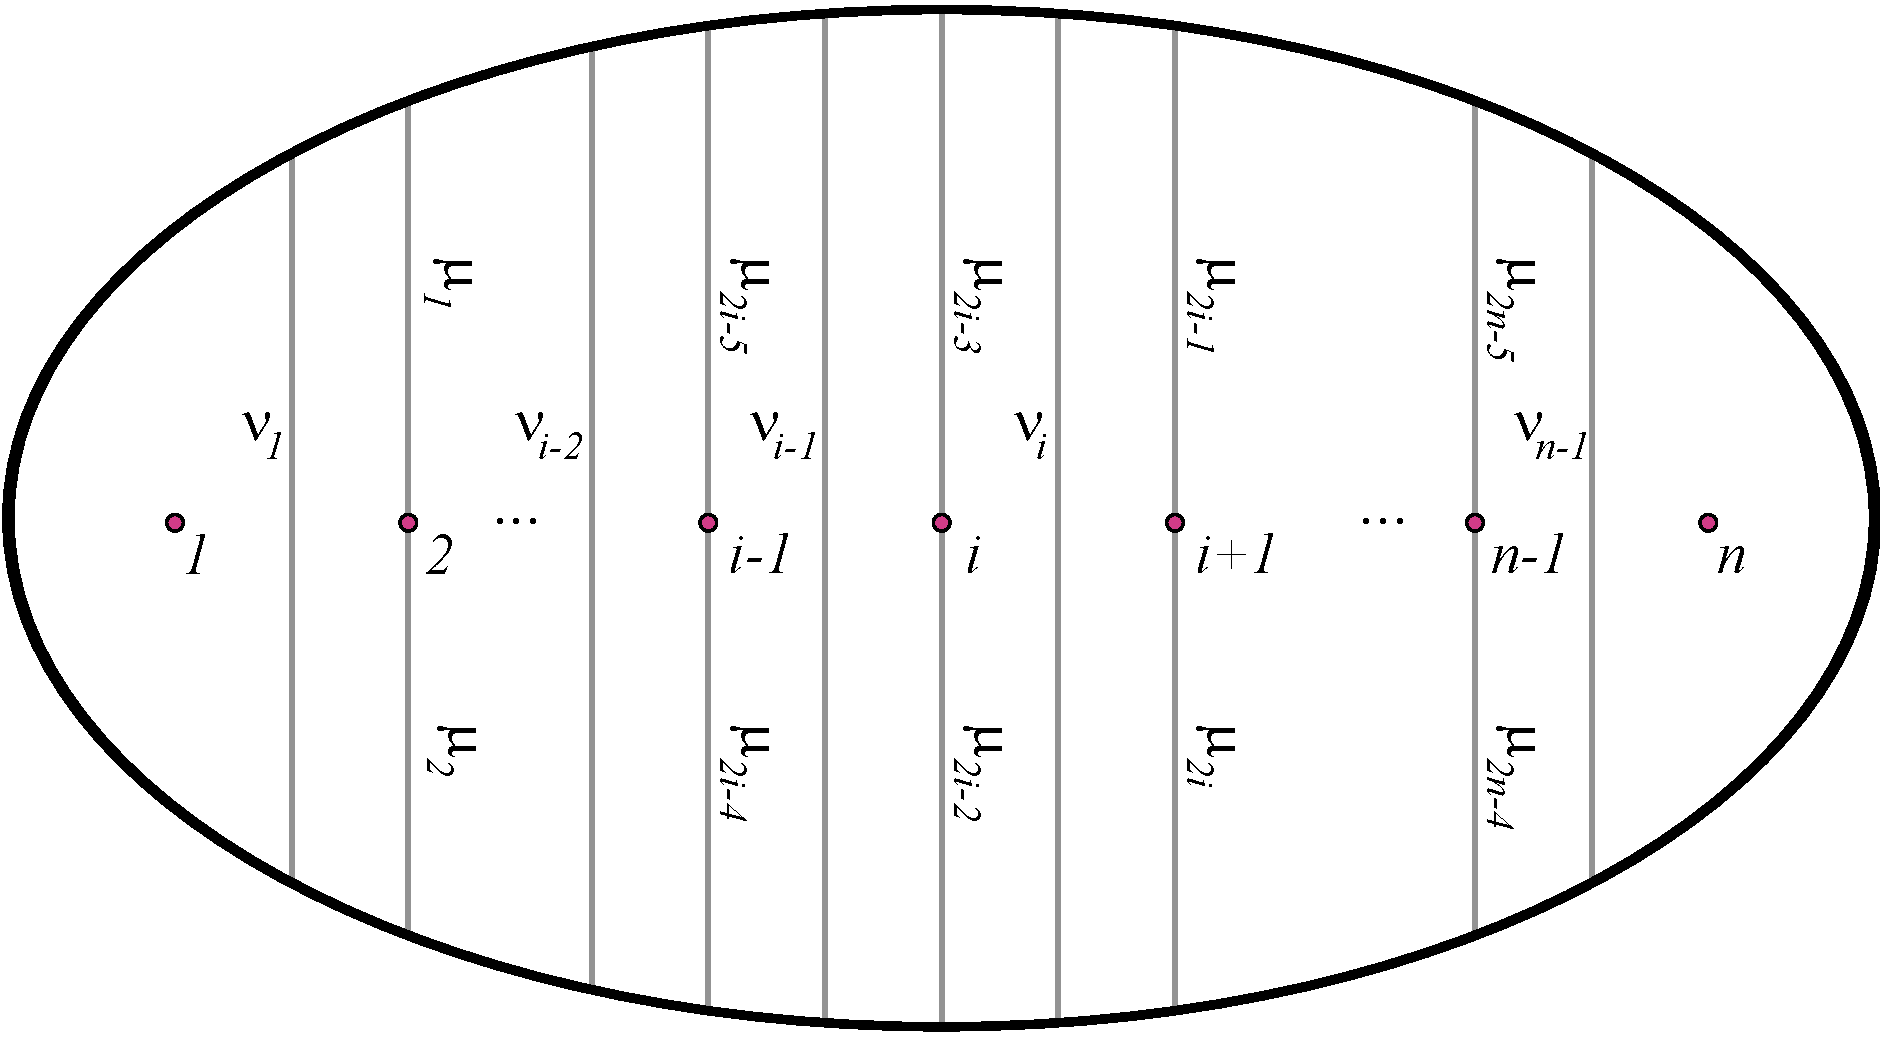
\includegraphics[height=.22\textheight]{dynn_def}
  \label{fig:dynn_def}
}
\end{center}
\caption{(a) A simple close loop in a disk with~$\nn=5$ punctures.
  (b) Definition of intersection numbers~$\mu_i$ and~$\nu_i$.
  [From~\citet{Thiffeault2010}.]}
\end{figure}
%
We consider equivalence classes of such loops under homotopies
relative to the punctures.  In particular, the loops are
\emph{essential}, meaning that they are not null-homotopic or
homotopic to the boundary or a puncture.  The \emph{intersection
  numbers} are also shown in Figure~\ref{fig:dynn_loop}: these count
the minimum number of intersections of an equivalence class of loops
with the fixed vertical lines shown.  For~$\nn$ punctures, we define
the intersection numbers~$\mu_i$ and~$\nu_i$ in
Figure~\ref{fig:dynn_def}.

Any given loop will lead to a unique set of intersection numbers, but
a general collection of intersection numbers do not typically
correspond to a loop.  It is therefore more convenient to define
\begin{equation}
  \ac_\ip = \tfrac12\l(\mu_{2\ip} - \mu_{2\ip-1}\r), \qquad
  \bc_\ip = \tfrac12\l(\nu_\ip - \nu_{\ip+1}\r), \qquad
  \ip=1,\ldots,\nn-2.
\end{equation}
We then combine these in a vector of length~$(2\nn-4)$,
\begin{equation}
  \abv = (\ac_1,\ldots,\ac_{\nn-2},\bc_1,\ldots,\bc_{\nn-2}),
  \label{eq:abvdef}
\end{equation}
which gives the \emph{loop coordinates} (or \emph{Dynnikov
  coordinates}) for the loop.  (Some authors such
as~\citet{Dehornoy2008} give the coordinates
as~$(\ac_1,\bc_1,\ldots,\ac_{\nn-2},\bc_{\nn-2})$.)  There is now a
bijection between~$\mathbb{Z}^{2\nn-4}$ and essential simple closed
loops~\citep{Dynnikov2002,Moussafir2006,Hall2009,Thiffeault2010}.
Actually, \emph{multiloops}: loop coordinates can describe unions of
disjoint loops. \jlt{MRA suggests `You mention multiloops here in a
  sort of fragment thought at the end of the second paragraph.
  Perhaps leave this concept out till section 2.4.'}

Let's create the loop in Figure~\ref{fig:dynn_loop} as a \loopc\ object:
\begin{lstlisting}[frame=single,framerule=0pt]
>> l = loop([-1 1 -2 0 -1 0])

l = (( -1 1 -2 0 -1 0 ))
\end{lstlisting}
Figure~\ref{fig:dynn_loop2} shows the output of the
\lstinline{plot(l)} command.  Now we can act on this loop with braids.
For example, we define the braid \lstinline{b} to be~$\sigma_1^{-1}$
with~$5$ strings, corresponding to the~$5$ punctures, and then act on
the loop \lstinline{l} by using the multiplication operator:
%
\begin{figure}
\begin{center}
\subfigure[]{
  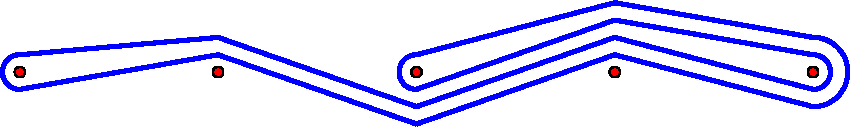
\includegraphics[width=.6\textwidth]{dynn_loop2}
  \label{fig:dynn_loop2}
}\hspace{1em}
\subfigure[]{
  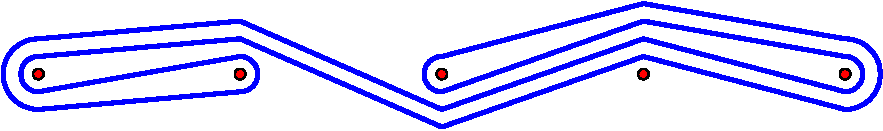
\includegraphics[width=.6\textwidth]{dynn_loop2_sigm1}
  \label{fig:dynn_loop2_sigm1}
}
\end{center}
\caption{(a) The loop \texttt{((-1 1 -2 0 -1 0))}.  (b) The braid generator
  $\sigma_1^{-1}$ applied to the loop in (a).}
\end{figure}
%
\begin{lstlisting}[frame=single,framerule=0pt]
>> b = braid([-1],5);   % one generator with 5 strings
>> b*l                  % act on a loop with a braid

ans = (( -1  1 -2  1 -1  0 ))
\end{lstlisting}
Figure~\ref{fig:dynn_loop2_sigm1} shows \lstinline{plot(b*l)}.  The
first and second punctures were interchanged counterclockwise (the
action of~$\sigma_1^{-1}$), dragging the loop along.

The minimum length of an equivalence class of loops is determined by
assuming the punctures are one unit of length apart and have zero
size.  After pulling tight the loop on the punctures, it is thus made
up of unit-length segments.  The minimum length is thus an integer.
For the loop in Figure~\ref{fig:dynn_loop2},
\begin{lstlisting}[frame=single,framerule=0pt]
>> minlength(l)

ans = 12
\end{lstlisting}
The \lstinline{entropy} method computes the topological entropy of a
braid by repeatedly acting on a loop, and monitoring the growth rate
of the loop.
\begin{lstlisting}[frame=single,framerule=0pt]
>> b = braid([1 2 3 -4]);
% apply braid 100 times to l, then compute growth of length
>> log(minlength(b^100*l)/minlength(l)) / 100

ans = 0.7637
>> entropy(b)

ans = 0.7672
\end{lstlisting}
The entropy value returned by \lstinline{entropy(b)} is more precise,
since that method monitors convergence and adjusts the number of
iterations accordingly.


\subsection{Loop coordinates for a braid}
\label{sec:loopcoords}

The loop coordinates allow us to define a unique normal form for
braids.  Consider the multiloop depicted in
Figure~\ref{fig:fundloops}, which is the output of \lstinline{plot(loop(5))}.
%
\begin{figure}
\begin{center}
\subfigure[]{
  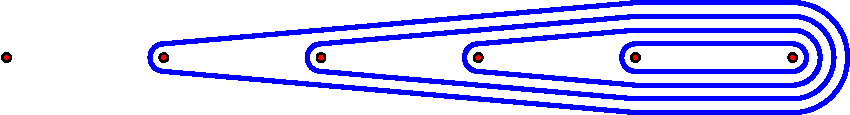
\includegraphics[width=.7\textwidth]{fundloops}
  \label{fig:fundloops}
}\hspace{1em}
\subfigure[]{
  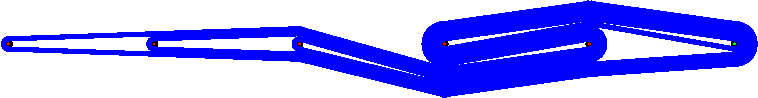
\includegraphics[width=\textwidth]{fundloops_act}
  \label{fig:fundloops_act}
}
\end{center}
\caption{(a) The multiloop created by \lstinline{loop(5)}.  (b) The
  multiloop \lstinline{b*loop(5)}, where \lstinline{b} is the braid
  $\sigma_1\sigma_2\sigma_3\sigma_4^{-1}$.}
\end{figure}
%
Notice that \lstinline{loop(5)} defaulted to a loop on a disk with $6$
punctures.  The reason is that this default multiloop is used to
define loop coordinates for braids.  The extra puncture is regarded as
the outer boundary of the disk, and the loops form a generating set
for the fundamental group of the disk with $5$ punctures.  The
canonical loops coordinates for braids exploit the fact that two
braids are equal if and only if they act the same way on the
fundamental group of the disk.  Hence, if we take a braid and act on
\lstinline{loop(5)},
\begin{lstlisting}[frame=single,framerule=0pt]
>> b = braid([1 2 3 -4]);
>> b*loop(5)

ans = (( 0  0  3 -1 -1 -1 -4  3 ))
\end{lstlisting}
then the set of numbers \lstinline{(( 0 0 3 -1 -1 -1 -4 3 ))} can be
thought of as \emph{uniquely} characterizing the braid.  It is this
property that is used to rapidly determine equality of
braids~\citep{Dehornoy2008}.  (The loop \lstinline{b*loop(5)} is
plotted in Figure~\ref{fig:fundloops_act}.)  The same loop coordinates
for the braid can be obtained without creating an intermediate loop
with
\begin{lstlisting}[frame=single,framerule=0pt]
>> loopcoords(b)

ans = (( 0  0  3 -1 -1 -1 -4  3 ))
\end{lstlisting}

\jlt{List of loops.}

\jlt{Next section: Braid from random walks?  Compute runs of same gen.}


\section{Side note: On filling-in punctures}

Recall the command~\texttt{subbraid} from Section~\ref{sec:braidclass}.  We
took the~$4$-string braid~$\sigma_1\sigma_2\sigma_3^{-1}$ and discarded the
third string, to obtain~$\sigma_1\sigma_2^{-1}$:
\begin{lstlisting}[frame=single,framerule=0pt]
>> a = braid([1 2 -3]);
>> b = subbraid(a,[1 2 4])   % discard string 3, keep 1,2,4

b = < 1 -2 >
\end{lstlisting}
%
\begin{figure}
\begin{center}
\subfigure[]{
  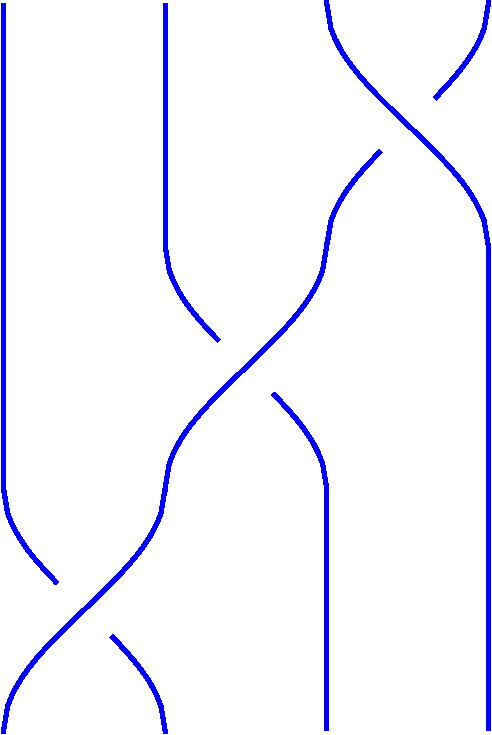
\includegraphics[width=.22\textwidth]{s1s2s-3_diagram}
  \label{fig:s1s2s-3_diagram}
}\hspace{5em}
\subfigure[]{
  
\includegraphics[width=.22\textwidth]{s1s-2_diagram}
  \label{fig:s1s-2_diagram}
}
\end{center}
\caption{Removing the third string from the braid
  (a)~$\sigma_1\sigma_2\sigma_3^{-1}$ yields the braid
  (b)~$\sigma_1\sigma_2^{-1}$.}
\end{figure}
\label{fig:subbraid}
%
The braids \texttt{a} and \texttt{b} are shown in Fig.~\ref{fig:subbraid};
their entropy is
\begin{lstlisting}[frame=single,framerule=0pt]
>> a.entropy, b.entropy

ans = 0.8314
ans = 0.9624
\end{lstlisting}
Note that the entropy of the subbraid~\texttt{b} is \emph{higher} than the
original braid.  This is counterintuitive: shouldn't removing strings cause
loops to shorten, therefore lowering their growth?\footnote{In fact, the
  entropy obtained by the removal of a string is constrained by the minimum
  possible entropy for the remaining number of strings
  \citep{LanneauThiffeault2011_braids}.  So here the entropy of the 3-braid
  could only be zero or $\ge 0.9624$.}

In some sense this must be true: consider the mixing device shown in
Fig.~\ref{fig:s1s2s-3_no_text}, where the rods move according the to
braid~$\sigma_1\sigma_2\sigma_3^{-1}$.
%
\begin{figure}
\begin{center}
\subfigure[]{
  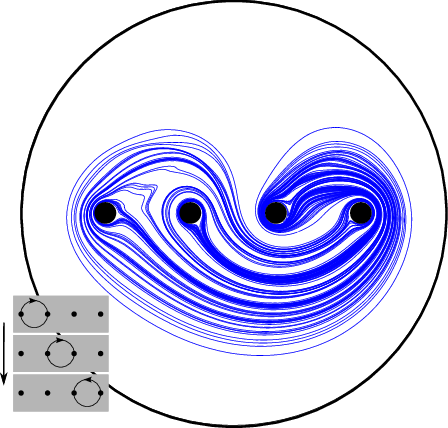
\includegraphics[height=.3\textheight]{s1s2s-3_no_text}
  \label{fig:s1s2s-3_no_text}
}\hspace{2em}
\subfigure[]{
  
\includegraphics[height=.3\textheight]{s1s2s-3_4_diagram}
  \label{fig:s1s2s-3_4_diagram}
}\hspace{2em}
\subfigure[]{
  
\includegraphics[height=.3\textheight]{s1s-2s1s-2s1s2_diagram}
  \label{fig:s1s-2s1s-2s1s2_diagram}
}
\end{center}
\caption{(a) The mixing device described by the
  braid~$\sigma_1\sigma_2\sigma_3^{-1}$ \citep{Thiffeault2008b}.  The inset
  shows how the rods are moved.  (b) The pure
  braid~$(\sigma_1\sigma_2\sigma_3^{-1})^4$.  (c)~The
  braid~$(\sigma_1\sigma_2^{-1})^2\sigma_1\sigma_2$, obtained by removing the
  third string from~(b).}
\label{fig:s1s2s-3_no_text}
\end{figure}
%
Removing the third string can be regarded as \emph{filling-in} the third
puncture (rod); clearly then the material line can be shortened, leading to a
decrease in entropy.

The flaw in the argument is that even though we can remove any string, we
cannot fill in a puncture that is permuted, since the resulting braid does not
define a homeomorphism on the filled-in surface.  To remedy this, let us take
enough powers of the braid~$\sigma_1\sigma_2\sigma_3^{-1}$ to ensure that the
third puncture returns to its original position, using the method
\texttt{perm} to find the permutation induced by the braid:
\begin{lstlisting}[frame=single,framerule=0pt]
>> perm(a)

ans = 2     3     4     1
\end{lstlisting}
The permutation is cyclic (it can be constructed with exactly one cycle), so
the fourth power should do it:
\begin{lstlisting}[frame=single,framerule=0pt]
>> perm(a^4)

ans = 1     2     3     4
\end{lstlisting}
This is now a \emph{pure} braid: all the strings return to their original
position.  Now here's the surprise: the subbraid obtained by removing the
third string from \texttt{a\^{}4} is
\begin{lstlisting}[frame=single,framerule=0pt]
>> b2 = (subbraid(a^4,[1 2 4]))

b2 = < 1 -2  1 -2  1  2 >
\end{lstlisting}
which is \emph{not} \texttt{b\^{}4}!  However, now there is no paradox in the
entropies:
\begin{lstlisting}[frame=single,framerule=0pt]
>> entropy(a^4), entropy(b2)

ans = 3.3258

Warning: Failed to converge to requested tolerance; braid is likely finite-order or has low entropy.
> In braid.entropy at 89

ans = 0
\end{lstlisting}
\braidlab\ has trouble computing the entropy because the braid \texttt{b2}
appears to be finite-order.  Indeed, the braid \texttt{b2} is conjugate
to~$\sigma_1^2$:
\begin{lstlisting}[frame=single,framerule=0pt]
>> c = braid([2 -1],3)

c = < 2 -1 >
>> compact(c*b2*c^-1)

ans = < 1  1 >
\end{lstlisting}
showing that its entropy is indeed zero.

The moral is: when filling-in punctures, make sure that the strings being
removed are permuted only among themselves.  For very long, random braids, we
still expect that removing a string will decrease the entropy, since the
string being removed will have returned to its initial position many times.


\section*{Acknowledgments}

The development of \braidlab\ was supported by the US National Science
Foundation, under grants DMS-0806821 and CMMI-1233935.  The author
thanks Michael Allshouse for extensive testing, comments, and for
contributing some of the code.  James Puckett and Karen Daniels
provided the test data from their granular medium
experiments~\citep{Puckett2012}.  \braidlab\ uses Toby Hall's
\emph{Train} \citep{HallTrain}; Jae Choon Cha's \emph{CBraid}
\citep{CBraid}; Juan Gonz\'{a}lez-Meneses's \emph{Braiding}
\citep{Braiding}; and Markus Buehren's \emph{assignmentoptimal}
\citep{assignmentoptimal}.


\bibliographystyle{jfm}
\bibliography{braidlab_guide}

% \lstinputlisting[lastline=50]{+braidlab/@braid/braid.m}

\end{document}
